\section{Brief report}

	\noindent Dear Officer:
	
	\noindent We understand that you are looking for a welding robot for the automotive industry and our team has found our product to be the right fit for your needs. I will then briefly describe our robot and show its advantages in terms of design and precision.
	
	\noindent We have designed a \textbf{four-armed robot} according to your requirements and have \textbf{considered its parameters}, which you can see in Table \ref*{T 2.1} and Table \ref*{T 2.2}. After simulation analysis, this design is reasonable and can perform the task accurately in the working area. We have also created a \textbf{kinematic diagram} (Figure \ref{F 4.1}) and a \textbf{workspace diagram} (Figure \ref{F 3.1}). At the same time, this four-armed robot also has \textbf{greater stability} and a \textbf{larger working area}.
	
	\noindent In terms of the \textbf{working path}, we have innovatively added a \textbf{one-second stabilization time}, which will make the work more stable. In the simulation, we set a 48-second working time which can be adjusted according to the specific situation. Figure \ref{F 5.3}  is a \textbf{schematic diagram} of the work.
	
	\noindent In Simulink, we conducted a detailed analysis of the errors. The maximum error in end effector position on the \textbf{x and z axes} is \textbf{below 0.05}, while the maximum error on the \textbf{y axis} is slightly \textbf{over 0.10}, and the largest error of joint angle is joint 2 angle, and it just nearly \textbf{reaches 0.02}. This indicates that the robot's motion and working process far exceed the standard accuracy. You can see the specific error images in Figure \ref{F 5.11} and Figure \ref{F 5.12}.
	
	\noindent Taking these advantages into account, I believe that our product is worth purchasing for your company and will bring substantial benefits. Next are the detailed design aspects of the robot.

\section{Introduction}
\FloatBarrier % Now figures cannot float above section title

Our product is a type of mechanical equipment used for automated welding. Our robotic arm can be widely used in various welding operations in the manufacturing industry, including automotive manufacturing, aerospace, construction, and manufacturing.

Our product has many adavantages. Firstly, it can improve production efficiency and quality by reducing the negative impact of human factors on production through automated welding operations. Secondly, it can reduce the danger of the work environment. 

In summary, the four-arm welding robot is an efficient and accurate welding device with many advantages. It will become an important part of automated production in the manufacturing industry, providing a reliable solution for various production operations.









\iffalse
The purpose of this experiment is to investigate the behaviour of a mild steel portal frame model when subjected to increasing loads.

The rig consists of a loading system that applies a vertical load at the center of the beam and a horizontal load at the top of one column. As shown in \autoref{f0}.

\begin{figure}[htbp]
    \centering
    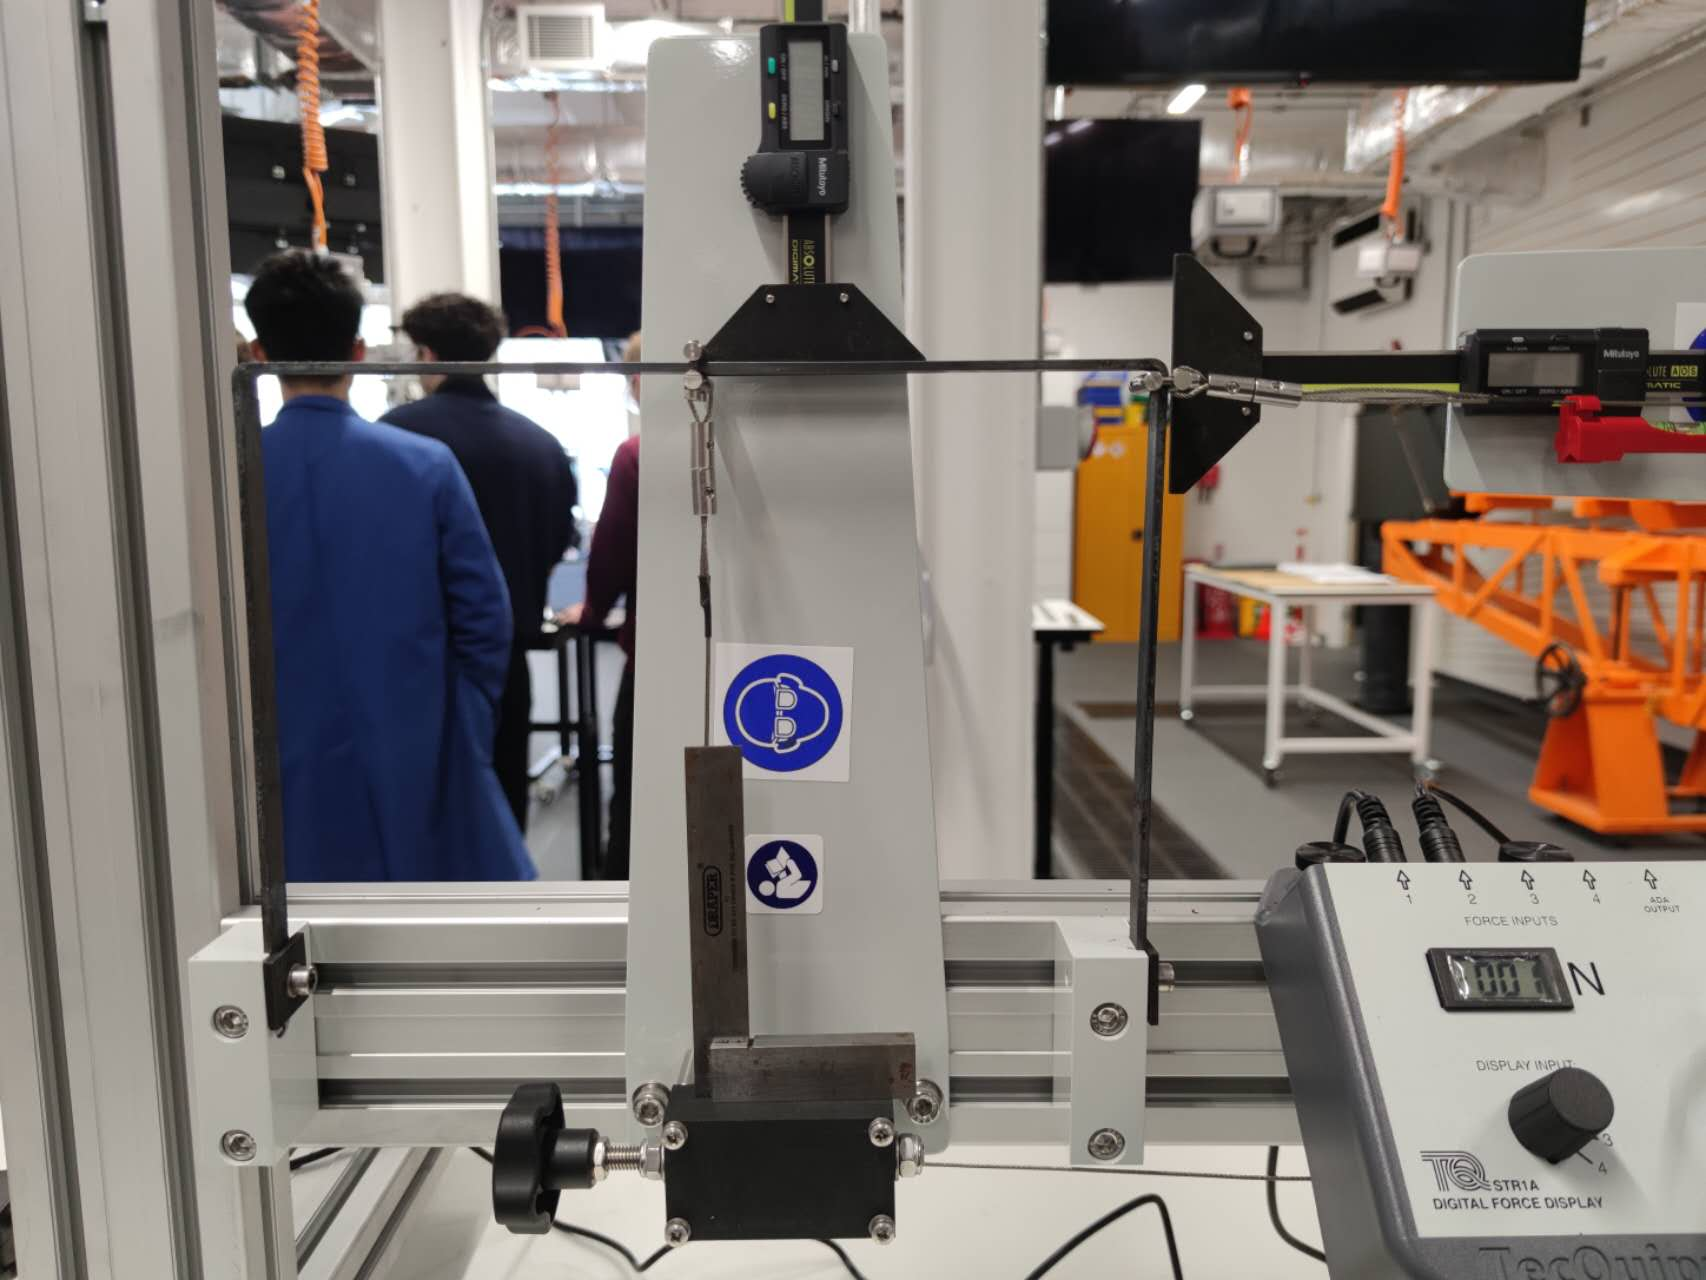
\includegraphics[width=7.5cm]{./fig/00.jpg}
    \caption{Experimental procedure}
    \label{f0}
\end{figure}

\fi


